\section{Configuration Selection}
\label{app:config}

\paragraph{Selection criterion.}
We select among 40 candidates spanning 4 feature dimensions and 10 window sizes. All candidates are evaluated only within the outer Training set via nested validation; the nine-task macro Significant-SDC F1 is the sole selection and ranking metric, and neither the internal Validation set nor the Test set participates. Figure~\ref{fig:config_matrix} (left) gives the complete 4$\times$10 matrix; the right panel re-scores the same candidate predictions against the fixed all-finite reference of the final 36D/$K{=}28$ configuration as an all-finite conditional diagnostic. Table~\ref{tab:A3} reports macro metrics at fixed $K{=}28$, and Figure~\ref{fig:window_ablation} gives window curves for both all retained executions and the all-finite subset at fixed 36D.

\begin{figure}[!ht]
\centering
    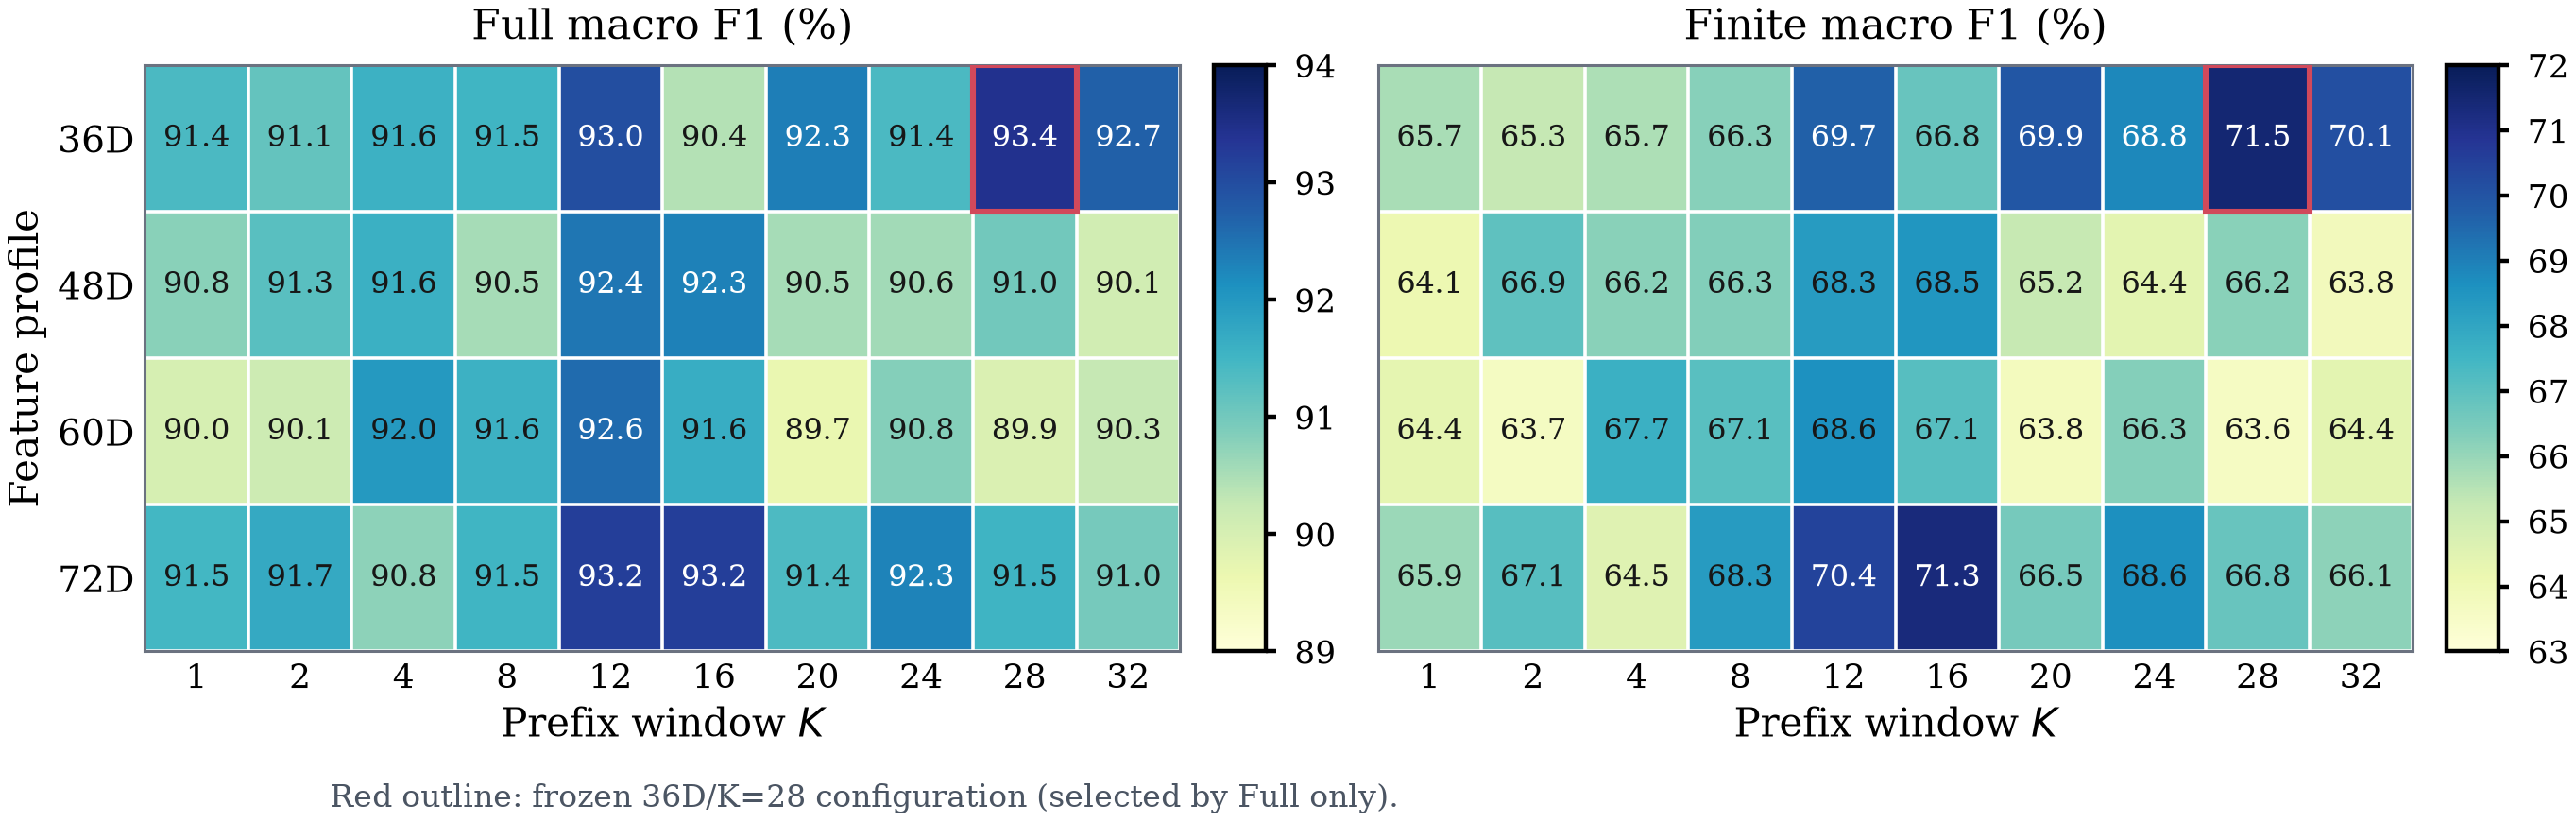
\includegraphics[width=1.0\linewidth]{Figures/figure8_configuration_F1_matrix.png}
    \caption{Training-only 4$\times$10 configuration-selection diagnostic. Left: nine-task macro Significant-SDC F1, the only result used for candidate selection and ranking; right: macro F1 scored on the fixed subset with all 36 features finite, after configuration freezing. Red boxes mark the 36D/$K{=}28$ selected and frozen by the primary metric; the two panels use independent color ranges.}
    \label{fig:config_matrix}
\end{figure}

\begin{table}[!ht]
\caption{Training-only macro metrics (\%) by feature dimension at fixed $K{=}28$.}
\label{tab:A3}
\centering
\small
\begin{tabular}{lcccc}
\toprule
\textbf{Feature} & \textbf{Precision} & \textbf{Recall} & \textbf{F1} & \textbf{FPR} \\
\midrule
\textbf{36D} & \textbf{99.17} & \textbf{88.66} & \textbf{93.42} & \textbf{0.028} \\
48D & 93.66 & 88.99 & 91.00 & 0.192 \\
60D & 92.77 & 88.22 & 89.93 & 0.270 \\
72D & 95.04 & 88.68 & 91.52 & 0.137 \\
\bottomrule
\end{tabular}
\end{table}

\begin{figure}[!ht]
\centering
    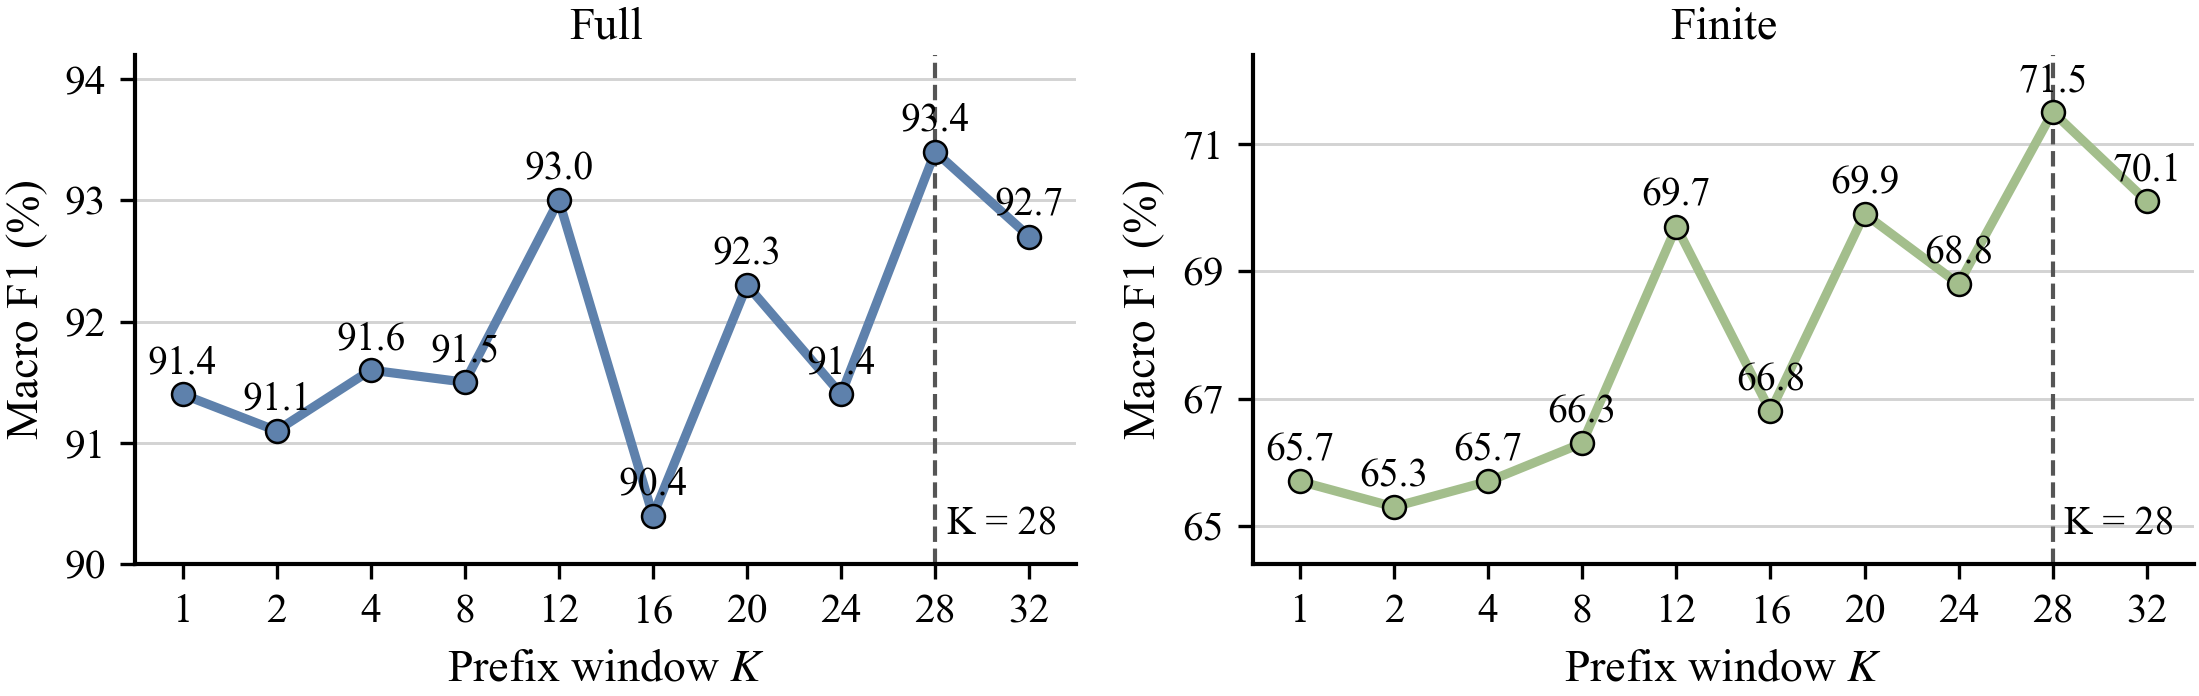
\includegraphics[width=1.0\linewidth]{Figures/figure9_window_ablation_F1.png}
    \caption{Training-only prefix-window diagnostic at fixed 36D. Left: macro F1; right: macro F1 scored on the fixed all-finite subset after configuration freezing. Each point is annotated with F1 (\%); dashed lines mark $K{=}28$ selected by the primary metric.}
    \label{fig:window_ablation}
\end{figure}

Fixed at $K{=}28$, 36D attains the highest F1 and the lowest FPR. The left panel of Figure~\ref{fig:window_ablation} shows that at fixed 36D, $K{=}28$ reaches the highest F1 (93.42\%); the right-side all-finite diagnostic likewise peaks at $K{=}28$ (71.49\%). We therefore freeze 36D/$K{=}28$, with the all-finite filter serving only as a post-freeze conditional diagnostic.

\paragraph{Post-freeze all-finite diagnostic.}
After configuration freezing, we run a conditional diagnostic within the same nested validation using the fixed 36D/$K{=}28$ all-finite reference vector. The filter changes only scored rows; training and threshold calibration are unchanged. Table~\ref{tab:A4} therefore explains performance under the numerically finite condition and plays no role in selecting or ranking the 40 candidates.

\begin{table}[!ht]
\caption{Training-only diagnostics of the frozen 36D/$K{=}28$ configuration on all retained executions and the all-finite subset (nine-task macro, \%).}
\label{tab:A4}
\centering
\small
\begin{tabular}{lcccccc}
\toprule
\textbf{Scope} & \textbf{Rows / Sig. SDC} & \textbf{Precision} & \textbf{Recall} & \textbf{F1} & \textbf{FPR} \\
\midrule
All & 53{,}076 / 1{,}912 & 99.17 & 88.66 & 93.42 & 0.028 \\
All-finite & 51{,}753 / 589 & 94.86 & 60.16 & 71.49 & 0.028 \\
\bottomrule
\end{tabular}
\end{table}

